\documentclass{article}
\usepackage[utf8]{inputenc}
\usepackage{amsmath}

\title{Terra Stability Analysis}
\author{\{nick, do\}@terra.money}
\date{\today \\v0.0.1}


\usepackage{natbib}
\usepackage{graphicx}
\graphicspath{ {images/} }
\usepackage{pgfplots}
\pgfplotsset{compat=1.15}

\begin{document}

\maketitle

\section{Introduction}

The purpose of this document is to analyze the stability of the Terra Protocol, in light of two foundational constraints that we are committed to: usability and decentralization. Terra is designed to be first and foremost a transactional currency, and we expect its use as a seamless and stable medium of exchange to dominate the high growth phase. We argue that Terra is best modeled as a decentralized payment network during this period, and that existing payment networks best resemble the dynamics of the Terra economy on its path towards becoming a mainstream currency. We demonstrate that the protocol maintains stability by leveraging Luna, Terra's collateral asset, even in the face of price shocks and precipitous falls in demand. We provide a framework for an additional layer of stability via a centralized fiat reserve during the early days of the protocol, as well as a framework for weaning off of it. Finally we outline areas of ongoing and future research.

\section{Demand Stickiness of Payment Networks}

Once consumers lock into a means of payment, they rarely switch to others - becoming “sticky.” The steady growth of payment networks like Visa, Amex and PayPal demonstrate the stickiness of payment networks, and by extension of the transaction volume that goes through them. The volatility of earnings for payment companies is very low, and prices are less volatile than the market benchmark (Figures 1 and 2). More importantly, stickiness and low volatility have significant implications when payment networks are viewed as standalone economies. The transaction volume that goes through a network is roughly proportional to “demand” in the virtual network economy. If the network used its own internal currency, this would directly translate to demand for the currency: higher transaction volume implies higher demand for the currency needed to fuel the economy, assuming roughly constant velocity of money in the network. \textbf{We are thus justified in reasoning about demand in a payments economy via earnings, which are just a proxy for transaction volume.}

It is clear that Terra functions like a decentralized payment network, and is in fact collateralized by the very shares of the network (Luna), which receive transaction fees as dividends. We expect high transaction/demand stickiness in the Terra economy after some threshold in adoption for all the reasons we mentioned earlier. We discuss ways to measure the threshold in a later section.  \textbf{The implications of demand stickiness are low churn, low volatility and consequently high earnings multiples for Luna. We collateralize Terra with an asset that receives a sticky revenue stream and derives its value from the high transactionality of the currency.} We later provide a quantitative version of this argument, demonstrating low volatility by modeling it as a function of churn likelihood. We use those properties in our analysis, making significantly more conservative assumptions compared to existing networks until we have grown in adoption. \textbf{The demand profile of Terra is in stark contrast to demand for speculative assets such as gold and (much more) Bitcoin, the latter two having no intrinsic value, no stickiness and thus being significantly more volatile.} A comparison between the volatility of Visa earnings and of the price of gold illustrates the argument nicely.  We consider the volatility of gold a best-case scenario for the volatility of bitcoin long-term (Figure 3).

Demand stickiness and low volatility have important implications on our stability analysis. They form the basis for valuing Luna, provide a framework for decommissioning the fiat reserve and demonstrate that transaction fees will be consistently low with rare exceptions.



\begin{figure}
	\centering
	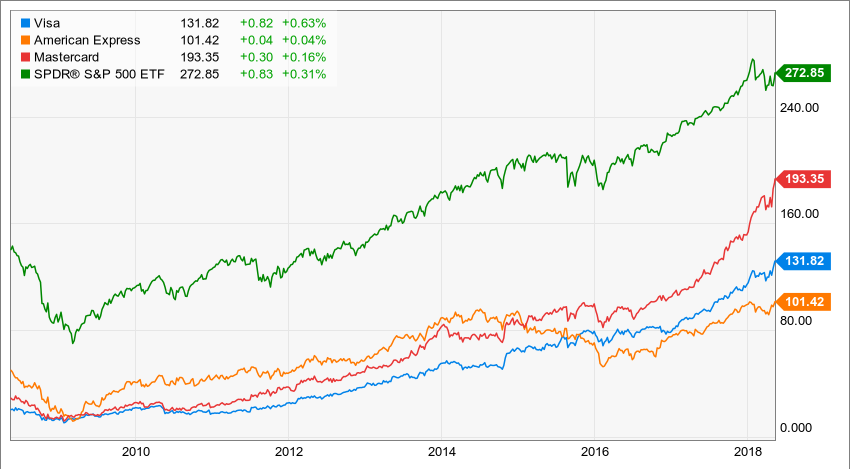
\includegraphics[scale=0.35]{fig1.png}
	\caption[]
	{VISA/AMEX/Mastercard price compared to SP 500 2008-2018}
\end{figure}


\begin{figure}
	\centering
	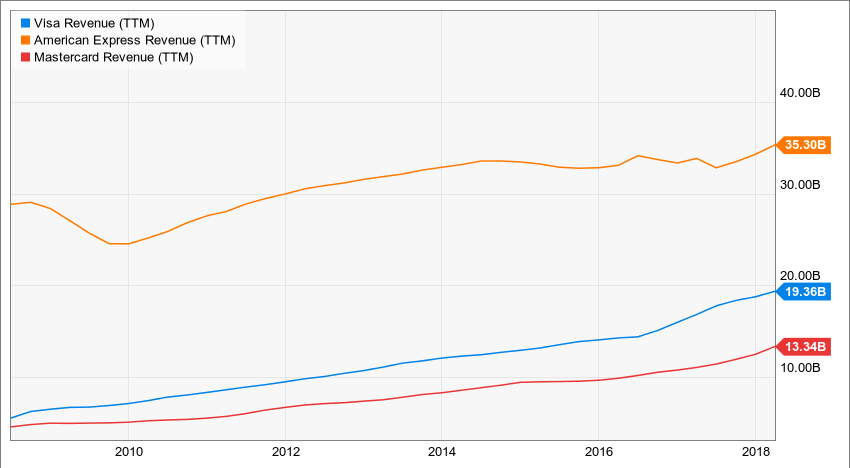
\includegraphics[scale=0.35]{fig2.png}
	\caption[]
	{AMEX, Visa, Mastercard revenues 2008-2018}
\end{figure}

\begin{figure}
	\centering
	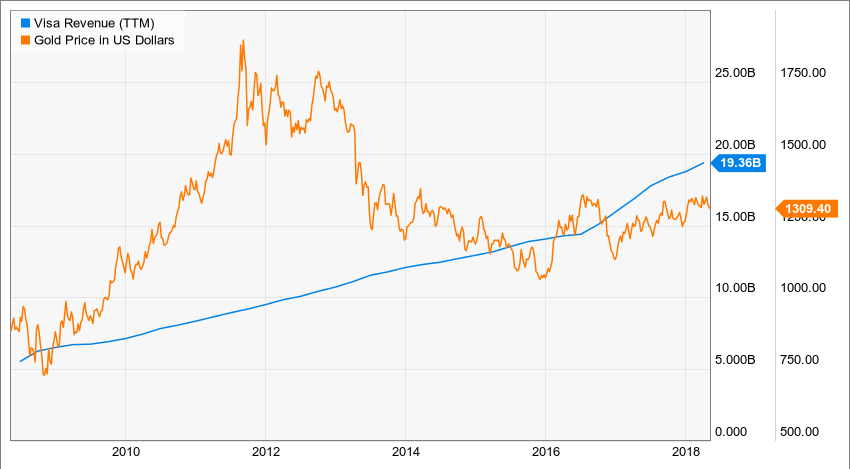
\includegraphics[scale=0.35]{fig3.png}
	\caption[]
	{Visa earnings compared to the price of gold 2008-2018}
\end{figure}


\newpage

\section{Guarantee of Solvency}

Terra remains stable insofar as we are able to sufficiently contract its supply during falls in demand or price shocks, or, in other words, if it remains solvent. We express solvency in the following equation:

\begin{center}
    Luna Reserve + Fiat Reserve ${>=}$ Terra Demand Drop (1)
\end{center}

Terra Demand Drop may in the worst case be the entirety of Terra's supply. Insofar as this equation holds during the lifetime of Terra, the system remains solvent hence the currency remains stable.

Recall that the Luna reserve is valued by discounting future transaction fee cash flows. This is described by the following equation: 

$$R_T = \sum_{t=T}^{\infty}\frac{f_tS_t}{(1+r)^t} \hspace{0.2cm} (2)$$ \newline

An equivalent formulation is via an earnings multiple on present transaction fee payouts:

 $$R_t = f_tT_tV_tm_t \hspace{0.2cm} (3)$$

\subsection{No Fiat Reserve}

We start by analyzing the steady state of our protocol, where there is no Fiat Reserve. After the Terra economy has entered maturity, we fully rely on the Luna Reserve for solvency. We analyze the process of decommissioning the Fiat Reserve in the next section. Recalling our earlier discussion, we note that at this stage comparisons to existing payment networks is legitimate — risk and return may be different, but we expect the risk/return profile to be on the same ballpark.

Let's explore the worst case for equation (1), where Terra's demand drop is close to 100\%. This is of course an extreme scenario for a relatively stable economy, but a crucial one nonetheless. This could be a coordinated Soros attack or a black swan event. In this case we need the Luna Reserve to be at least as valuable as Terra's supply if we are to stay solvent. Equation (3) simplifies to the following:

$$f_tV_tm_t >= 1 \hspace{0.2cm} (4)$$

To proceed with worst-case analysis in equation (4), we assume an earnings multiple $m_t$ of 5 — this is where Amex traded at the very bottom of the 2008 financial crisis after a calamitous 82\% drop in price (not revenue) in less than 2 years. This is the lowest multiple any of the major payment networks have traded at in their history (Visa, Mastercard, Amex, PayPal). Amex trades at a P/E of more than 100 as of May 2018. We assume a conservative money velocity of 10, this is a historical average for the velocity of the USD's M1 and we consider it a lower bound for Terra given its use in e-commerce which experiences much higher velocities. To satisfy equation (4) under those extreme conditions we need transaction fees of 2\%. This is on-par with the fees major e-commerce companies pay to Visa (e.g. TMON), and in fact approximately break-even for most payment networks given the numerous middlemen their infrastructure involves. 

\textbf{So Terra remains solvent in the most extreme conditions (no fiat reserve, near 100\% drop in demand, rock-bottom Luna earnings multiple) by charging fees on-par with competition.}

\subsection{Gradually Decreasing Fiat Reserve}

At genesis we maintain a 100\% fiat reserve that guarantees stability in the very early days during which volatility is expected and natural. As the Terra economy grows and volatility decreases we gradually wean off of the reserve. In what follows we outline the framework for decommissioning the reserve.

Earlier we argued that demand for payment networks like Terra is very sticky — businesses who start relying on Terra and consumers who develop spending habits tend to stick. We now present a quantitative version of this argument, considering the number of e-commerce companies using Terra, $n$, and the probability that any one company churns over a year, $p$. The number of e-commerce companies using Terra is a good proxy for Terra demand. We demonstrate that as $n$ grows (adoption) and $p$ drops (stickiness) the volatility of Terra demand drops very fast. We further quantify the probability that demand will fall below a given threshold and obtain high-probability bounds for it.

Observe that the number of companies to churn in a given year follows a Binomial distribution with parameters $n$ and $p$, and is closely approximated by a Normal distribution with mean $np$ and variance $np(1-p)$. The relative volatility of demand (volatility divided by $n$) is therefore $\frac{\sqrt{np(1-p)}}{n}$. As $n$ grows and $p$ decreases this value decreases rapidly. \textbf{Intuitively, all this says is that demand for Terra becomes very stable as adoption grows and churn likelihood decreases.}

We can easily obtain confidence intervals for demand using this model. To make this concrete let's explore possible scenarios for Terra adoption 1, 3 and 5 years from now, making aggressive assumptions about churn likelihood. To make this analysis statistically significant we consider e-commerce partners to be companies with significant transaction volume (\$1B+ in GMV).

\begin{center}
\begin{tabular}{ |c|c|c|c|c| } 
 \hline
Year & Tx vol (\$B) & Churn Prob \% & Max Demand Drop \% & Fiat Ratio \% \\
 \hline \hline
1 & 10 & 20 & 43 & 100 \\
\hline
3 & 60 & 10 & 21 & 20 \\
\hline
5 & 140 & 5 & 11 & 10 \\
 \hline
\end{tabular}
\end{center}


Note that the maximum drop in demand that we expect decreases as the number of partners increases and churn likelihood decreases. We can expect with high confidence, for example, that after 3 years drops in demand should not exceed 21\%. Some of the assumptions that this model makes will be false, so it will clearly not be fully accurate, but it delivers the main message, which is that demand for Terra is sticky and becomes stable quickly. We will be closely observing how churn probabilities evolve over time and how they impact volatility in Terra demand.

We set the schedule for decommissioning the fiat reserve in accordance with the volatility of demand for Terra, which we both model and measure historically. From equation (1) from the previous section, the Luna and Fiat Reserves in combination need to be more valuable than any demand drop to maintain solvency. \textbf{The guiding principle for the Fiat Reserve is to provide a buffer for large part of worst-case demand drops in the early years while the economy and markets are immature.} During the first year a 100\% fiat reserve will in fact cover much more than demand drops we expect — this added protection is desirable. In accordance with the estimates above, by year 3 we would maintain a 20\% fiat reserve, and by year 5 at most 10\%. After year 5 we would stop funding the fiat reserve, and would start spending it to fund further growth for Terra. The Foundation may maintain some fiat to provide a liquidity buffer to the Terra market, but that will eventually be a negligible fraction of Terra supply.

Beyond providing an additional layer of stability, which is all but guaranteed in combination with the Luna Reserve, \textbf{the Fiat Reserve acts as a subsidy to transaction fees up to the point where the Luna Reserve can fund contractions using very low fees.} Say, for example, that there is a Black Swan demand drop of 40\% during year 5, even though our models and historical volatility suggest a drop of more than 10\% is highly unlikely. The Fiat Reserve is only 10\%, so the Luna Reserve is tasked with funding the remaining 30\%. Let's assume an earnings multiple of 5, which is very low given the relative maturity of the Terra economy at this point. From equation (3) above, using a velocity of 10, it follows that transaction fees of 0.6\% are sufficient to fund the demand drop. 

\section{Ongoing and Future Research}

\begin{itemize}
    \item Development of more sophisticated volatility models that will allow us to predict Terra demand volatility more accurately. This will be important in the process of decommissioning the Fiat Reserve.
    
    \item Further research on the impact of transaction fees on volume. We have argued that volume should see minimal change if transaction fees are lower than traditional payment networks. Are there case studies where high transaction fees in e-commerce hurt volume, or where younger competitors were able to steal volume because of lower fees?
    
    \item How do we refine our approach to fees and volatility estimation when Terra gains broad adoption outside of e-commerce (eg financial applications like escrow, credit markets etc)
    
    \item How do we optimize staking incentives for cold deposits depending on market conditions?
    
    \item Run simulations under a variety of market conditions and stress-test the protocol as much as possible. Vary parameters such as churn probability, earnings multiple and volatility to gauge impact on transaction fees and optimal fiat reserve.
\end{itemize}


\section{Conclusion}

We have demonstrated that the Terra protocol keeps Terra stable, usable and decentralized. In particular we have shown, both by comparison to existing payments networks and quantitatively, that Terra will develop significant demand stickiness as it gains adoption. We have proven that Terra remains solvent under the harshest market conditions with no fiat reserve and with fees on par with competition. We have further provided a framework for a gradually diminishing Fiat Reserve that guarantees very low transaction fees to Terra users throughout the early days of the economy.

\end{document}
